\documentclass[11pt,a4paper]{article}
\usepackage[T1]{fontenc}
\usepackage[utf8]{inputenc}
\usepackage{lmodern}
\usepackage[margin=25mm]{geometry}
\usepackage{microtype}
\usepackage{amsmath}
\usepackage{booktabs}
\usepackage{graphicx}
\usepackage{xcolor}
\usepackage[font=small,labelfont=bf]{caption}
\usepackage[colorlinks=true,linkcolor=blue!50!black,citecolor=blue!50!black,urlcolor=blue!50!black]{hyperref}
\usepackage{array}
\setlength{\parskip}{3pt}
\renewcommand{\arraystretch}{1.12}
\newcommand{\todo}[1]{\textcolor{red}{[#1]}}
\hypersetup{pdftitle={Laya-MLX as a Fast Local Decision Engine for Browser Automation},pdfauthor={Robert Keller},pdfkeywords={browser automation, element grounding, GUI testing, encoder models, Apple MLX, confidence cascades}}

\title{\textbf{Laya-MLX as a Fast Local Decision Engine for Browser Automation:\\ Element Grounding in Iframes, UI Tests and Live Sites on Apple Silicon}}
\author{Robert Keller\\ \small Independent researcher\\ \small \texttt{development@whocode.de}\\ \small ORCID: \href{https://orcid.org/0009-0003-0388-5246}{0009-0003-0388-5246}}
\date{Preprint, version 1 --- experiments conducted 5--6 November 2026}

\begin{document}
\maketitle

\begin{abstract}\noindent
Browser agents and instruction-driven UI tests spend most of their time and cost in a language-model call that chooses the next action. Laya is a small encoder (322M--421M parameters) that answers constrained questions---choose an option, score, judge true/false---in a single forward pass; \texttt{laya-mlx} runs it on Apple GPUs. We evaluate it as an \emph{element-grounding} engine: given an instruction and a page's interactive elements, which element should be used? Our open pipeline snapshots a page across iframes and open shadow DOM, asks Laya, and acts through Playwright. On an Apple M2 Pro we tested a todo app (original plus four UI mutations), a checkout flow with nested cross-origin iframes, shadow DOM and a canvas control, 19 steps on public sites (five runs), and a replay of 144 logged decisions (38 distinct instructions) through Laya, a lexical matcher, bge-m3 embeddings and a local Qwen3-8B model. With a frame-aware snapshot, the 322M Laya model completed every checkout step through nested cross-origin iframes (2/6 with a main-frame-only snapshot) and chose the correct element in all 94 live decisions (18 distinct decisions $\times$ 5 runs; median 51\,ms). On the 88 non-trivial replayed cases, top-1 accuracy was 67\% (322M) and 74\% (421M) versus 55\% for lexical matching, 74\% for embeddings and 82\% for the LLM; on a live page with 40 or more candidates Laya was no better than lexical matching. Laya's confidence was informative, and escalating uncertain decisions to the LLM gave 78.4\% (322M) and 86.4\% (421M) accuracy at 141 and 223\,ms, versus 81.8\% at 307\,ms for the LLM alone. Samples are small and no accuracy difference between grounders is significant after correction. We also report an idle-gap latency penalty and provide a replication package.
\end{abstract}

\noindent\textbf{Keywords:} browser automation; element grounding; GUI testing; small encoder models; Apple MLX; confidence-based cascades.

\section{Introduction}
Language-model agents that operate web pages spend most of their wall-clock time and money in the model call that selects each action. A large class of those decisions is narrow---\emph{which field is the destination, which button does this instruction refer to}---and does not need open-ended generation. Laya \cite{laya} is an open-weight encoder trained to answer such typed questions (\texttt{choice}, \texttt{score}, yes/no) with probabilities (described by its authors as calibrated) from a single bidirectional pass, and its MLX port \cite{lmlx} runs it natively on Apple GPUs without PyTorch. Its authors report median latencies of 13.4\,ms (English checkpoint) and 7.4\,ms (multilingual) for short decisions on an M3~Max \cite{lmlx}. Whether such a model is useful for \emph{real} browser automation---iframes, shadow DOM, changing UIs, third-party sites---we could not find reported; we did not perform an exhaustive literature search (Section~\ref{sec:limits}).

We ask six research questions (answered in the order RQ1, RQ2, \ldots). \textbf{RQ1:} Can a Laya-driven agent operate inside iframes (same-origin, cross-origin, nested) and shadow DOM? \textbf{RQ2:} How does instruction-driven testing with Laya compare with scripted CSS and role/text selectors when the UI changes? \textbf{RQ3:} Does it work on third-party pages we did not write? \textbf{RQ4:} How do its accuracy and latency compare with a lexical matcher, an embedding model and a local LLM, and how do they scale with the number of candidate elements? \textbf{RQ5:} Is its confidence a usable escalation signal? \textbf{RQ6:} How does it behave at runtime on Apple Silicon (compile flags, batching, idle gaps)?

\paragraph{Terminology.} \emph{Element grounding} means mapping an instruction (``Tick off Walk dog'') to the page element it refers to. A \emph{candidate} is an interactive element found on the page; the \emph{gold element} is the one that, when operated, achieves the instruction. A \emph{frame-aware snapshot} enumerates candidates in all frames; a \emph{main-frame-only snapshot} ignores iframes. \emph{Literal} instructions reuse the wording of the original UI; \emph{natural} instructions paraphrase it. A \emph{cascade} first asks Laya and escalates to the LLM when Laya's probability for its top choice is below a threshold; \emph{LOGO} (leave-one-group-out) chooses that threshold on all suite groups except the one being evaluated. \emph{Discriminative} cases are defined in Section~\ref{sec:protocol}.

\paragraph{Contributions.} (i) An open element-grounding pipeline (frame- and shadow-DOM-aware snapshot, Laya grounder, Playwright executor) and a set of test suites with gold labels. (ii) A paired comparison of Laya against three baselines on 144 logged decisions (38 distinct instructions; 88 decisions, 32 instructions, are discriminative), with instruction-level (cluster) confidence intervals and permutation tests. (iii) Scaling measurements of accuracy and latency up to 160 candidates on a live page. (iv) Evidence on whether Laya's confidence predicts correctness, and a leave-one-group-out evaluation of a Laya$\to$LLM cascade. (v) Runtime findings, including an idle-gap latency penalty and its mitigation. (vi) A replication package (see Data and code availability).

\section{Background and related work}
\paragraph{Laya and laya-mlx.} Laya \cite{laya} is a decision encoder whose architecture follows ModernBERT \cite{modernbert}; it generates no tokens, and returns probabilities for options (\texttt{choice}), ordered levels (\texttt{score}) or a yes/no proposition (\texttt{noul}). The independent MLX port \cite{lmlx} reimplements the encoder and heads on Apple's MLX framework \cite{mlx}. Three checkpoints are published: a 421M English model (512-token context), a 322M multilingual model (1{,}024 tokens; ``Laya-ML'' below) and a 421M ``typed-decisions'' model (1{,}024 tokens; ``Laya-TD''). The port reports agreement with upstream on 63/63 validation questions; this measures port fidelity, not task accuracy \cite{lmlx}.

\paragraph{Browser agents built on small decision models.} \texttt{jev-ultrafast} \cite{jev} is a fast browser agent that asks a hosted decision model for each action; \texttt{laya-ultrafast} \cite{layaultrafast} ports it to Laya, pairing narrow Laya questions with site-independent rules and one text-model call per task for planning. Its authors report that Laya does not reliably answer the open question of what the browser should do next, which motivates our narrower scope: we give Laya only element-selection questions and do not evaluate planning.

\paragraph{Baselines and tooling.} We compare against a lexical matcher, the multilingual embedding model BGE-M3 \cite{bgem3} and the LLM Qwen3-8B \cite{qwen3} served locally with Ollama \cite{ollama}. Browser control uses Playwright \cite{playwright}. We do not survey the wider literature on LLM-based web agents and self-healing test automation; see Section~\ref{sec:limits}.

\section{Method}
\subsection{Pipeline}
Figure~\ref{fig:pipeline} shows the pipeline. \emph{Snapshot:} for every frame (including cross-origin frames, evaluated out of process by Playwright) a script enumerates visible interactive elements---links, buttons, inputs, selects, ARIA roles, \texttt{contenteditable}, \texttt{onclick}, focusable nodes---recursing into \emph{open} shadow roots. Each element receives a \emph{name} (aria-label, associated label, text, title/placeholder/alt; an unlabeled checkbox takes its row's text) and a \emph{context} (the text of the enclosing row or card with its controls removed, so that a ``Delete'' button knows it belongs to ``Write report''). Native inputs hidden with CSS \texttt{opacity:0} are kept because they remain operable. \emph{Grounder:} given an instruction and the candidates, return one element. \emph{Executor:} act through a Playwright element handle in the correct frame (click; fill with the quoted text of the instruction; select an option, chosen by a second Laya question; optional Enter).

\begin{figure}[t]\centering
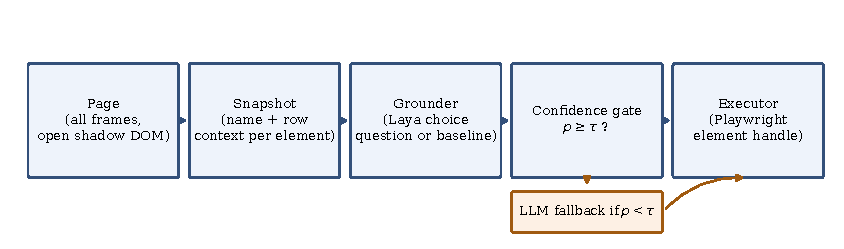
\includegraphics[width=\linewidth]{figures/fig_pipeline.pdf}
\caption{Pipeline. The confidence gate and LLM fallback are used only in the cascade experiments (Section~\ref{sec:cascade}).}\label{fig:pipeline}
\end{figure}

\subsection{Grounders}
\textbf{Laya choice} (Laya-ML, Laya-TD): one \texttt{choice} question whose options are \texttt{\{label: description\}} with a short unique label (the element name) and a longer description (role, name, row context); duplicate labels are disambiguated by row context, then by ordinal (e.g., ``(2 of 3)''). \textbf{Laya pointwise:} one yes/no question per candidate, all candidates packed into a single batched pass. \textbf{Lexical:} IDF-weighted overlap of lowercased tokens truncated to six characters (a crude stemmer) between instruction and element text. \textbf{Embedding:} BGE-M3 cosine similarity between instruction and each candidate. \textbf{LLM:} Qwen3-8B (4-bit quantized, thinking disabled, temperature~0, at most 8 output tokens) given a numbered candidate list and asked for one number. \textbf{Lexical-15 + Laya-ML} (scaling experiment only): the 15 candidates sharing the most (unweighted) tokens with the instruction, passed to Laya-ML. Exact prompts are in Appendix~\ref{app:prompts}. The LLM uses a single untuned prompt and was run once per case; stronger prompts or models would likely improve it. Scripted baselines were written once against UI variant~A in two styles: CSS selectors, and role/text locators (Playwright's recommended style). \textbf{Which Laya model drove the end-to-end suites:} the todo, checkout and live suites (Tables~\ref{tab:shop}--\ref{tab:live}) were executed with Laya-ML (322M); Laya-TD and all baselines were evaluated by replaying the logged cases (Section~\ref{sec:protocol}).

\subsection{Test suites}\label{sec:suites}
\textbf{Todo (local).} A task app, seven steps (type, add, toggle one item, delete one item, two filters, clear completed), each with a literal instruction written against variant~A wording and a natural paraphrase (Appendix~\ref{app:instr}), on five UI variants: A (baseline) and four mutations: B (obfuscated classes/ids, shuffled control order); C (relabeled visible text); D (icon-only buttons with aria-labels); E (icon-only, no accessible name; a negative control). State is reset before each step and success is read from application state, not the DOM. \textbf{Checkout (local).} Add item, open checkout, enter name and card number (dummy values), choose country, pay; the payment form is inline, in a same-origin iframe, a cross-origin iframe, or nested iframes, with plain fields, \emph{open} shadow DOM, \emph{closed} shadow DOM, or a canvas-drawn Pay button (11 conditions), run with a frame-aware and a main-frame-only snapshot. \textbf{Live.} 19 steps on public pages: nine tasks on the-internet.herokuapp.com \cite{theinternet} (checkboxes, dropdown, add/remove, dynamic loading, JS confirm, number input, status-code links, a 25-link table with duplicate ``edit''/``delete'' links, a TinyMCE editor in an iframe) and, as the tenth task, the React TodoMVC app \cite{todomvc} (seven steps; 12 + 7 = 19 steps in all); no logins or personal data. \textbf{Scaling (live).} The English Wikipedia article ``Alan Turing'': 264 unique article links remained after filtering; each trial uses the target link plus $N{-}1$ random distractors, $N\in\{5,10,20,40,80,160\}$, five targets $\times$ two instruction styles $\times$ three samples (30 trials per cell). The natural instructions describe the target indirectly (e.g., ``the page about his doctoral supervisor at Princeton'') and therefore require world knowledge, not only UI understanding.

\begin{table}[t]\centering\small
\begin{tabular}{@{}lp{12.2cm}@{}}\toprule
Hardware & Apple M2 Pro, 16\,GB unified memory; macOS 27.0.1 (build 26A434)\\
Laya & \texttt{laya-mlx} 0.6.0, MLX 0.32.4; checkpoints \texttt{aac6fef/laya-multilingual-mlx} (rev.\ \texttt{f2b4faf}) and \texttt{aac6fef/laya-typed-decisions-mlx} (rev.\ \texttt{f9e501c}), FP16\\
Browser control & Playwright (Python) 1.64.1, Google Chrome 156 (headless); Python 3.12.13\\
Baselines & Ollama 0.40.13; \texttt{qwen3:8b} (8.2B, Q4\_K\_M, digest \texttt{500a1f067a9f}); \texttt{bge-m3} (567M, F16, digest \texttt{790764642607})\\
\bottomrule\end{tabular}
\caption{Experimental environment.}\label{tab:env}
\end{table}

\subsection{Gold labels, logging and evaluation sets}\label{sec:protocol}
Each step has a gold element (a test attribute in local fixtures; a predicate over role, name and context on live pages, written by the author). After a failed step the harness executes the gold element so later steps are measured independently (``oracle resync''); todo steps start from a reset state. Every (instruction, candidate list, gold) triple from the Todo, Checkout (frame-aware) and Live runs was logged---144 cases with a gold element present---and replayed through all grounders, each in its own process so that models do not compete for memory. The 144 cases are \emph{not} 144 independent problems: they comprise \textbf{38 distinct instructions} (14 todo step--style pairs, 6 checkout steps, 18 live steps), each repeated across the five todo variants or the checkout conditions. The cases split into 14 development cases (todo variant~A), 56 todo cases on variants B--E, 56 checkout cases (3--8 candidates each) and 18 live cases. Because every grounder solved all 56 checkout cases, we designate them \emph{non-discriminative} and call the remaining 88 cases (32 distinct instructions) \emph{discriminative}; this designation was made \emph{after} seeing the results, so we report both sets and treat the 88-case figures as primary. \emph{Warm latency} is the median over a second pass through the same inputs (so compiled shapes, Laya's prompt cache and Ollama's prompt cache may all be warm); it excludes the page snapshot. The 95th percentile is the order statistic at index $\lfloor0.95(n-1)\rfloor$. Todo variant~A served as the \emph{development set} on which option formatting, question wording and the pointwise/choice formulation were compared (Appendix~\ref{app:dev}); all other suites are held out for those choices. We fixed two harness defects after observing live failures (CSS-hidden native checkboxes were not enumerated; one check could pass spuriously), so the live suite is not held out with respect to the snapshot and its checks; these fixes changed the snapshot and the check, not Laya's prompts.

\subsection{Statistics}
Because cases within an instruction are strongly dependent, confidence intervals for accuracy are \emph{cluster-bootstrap} percentile intervals (10{,}000 resamples of instructions with all their cases). Paired comparisons use a sign-flip permutation test over per-instruction differences (20{,}000 permutations), with Holm adjustment over all 15 grounder pairs; we report them on the 88 discriminative cases. Wilson intervals \cite{wilson} are used only for single proportions in the text (Section~4.3). The LOGO cascade chooses its threshold from $\{0.5,0.6,0.7,0.8,0.9,0.95\}$ by maximizing accuracy on the training groups (ties to the lower threshold); groups are development, todo B--E and live, plus checkout in the 144-case version. Cascade latency is each case's Laya latency plus the LLM latency when the case is escalated. The end-to-end suites were repeated (todo and checkout $\times3$, live $\times5$).

\subsection{Environment}\label{sec:env}
Table~\ref{tab:env} lists the software and hardware. Laya ran with \texttt{compile=True}, \texttt{pad\_to\_multiple=16}, \texttt{cache\_prompts=True} unless stated (``default'' below means none of these flags). \textbf{A measurement confound:} in a first protocol, with Laya, an LLM and an embedding model resident at once on the 16\,GB machine, swap exceeded 20\,GB and some latencies inflated by one to two orders of magnitude. The reported timings come from a second protocol with less contention: one model family per process and Ollama models unloaded before Laya runs. This does not guarantee a quiet machine: macOS still reported 8--23\,GB of swap in use during some second-protocol runs (possibly stale pages from earlier activity), so timings are indicative, and repeated Ollama latency measurements at large $N$ differed by up to a factor of six between runs (Section~\ref{sec:scale}). The replayed accuracies of the six grounders were unchanged between the two protocols (the first-protocol logs are not included in the replication package).

\section{Results}
\subsection{Iframes, shadow DOM and canvas (RQ1)}
With a frame-aware snapshot, Laya-ML completed all six checkout steps through same-origin, cross-origin and nested iframes and through open shadow DOM, in all three repeats; with a main-frame-only snapshot the flow stopped after two steps whenever the form was in an iframe (Table~\ref{tab:shop}). Closed shadow roots and canvas-drawn controls are invisible to DOM enumeration, so the flow stopped there regardless of the grounder. Laya chose the gold element in every step whose gold element was present (56/56). This suite does \emph{not} discriminate between grounders: all of them, including the lexical matcher, scored 56/56, because each step has three to eight distinctly labeled candidates, and the main-frame-only result is true by construction (the elements are never enumerated). It tests the snapshot and executor, not the model.

\begin{table}[t]\centering\small
\begin{tabular}{lrr}
\toprule
Payment form location & All-frames snapshot & Main-frame-only \\
\midrule
Inline form & 6/6 & 6/6 \\
Same-origin iframe & 6/6 & 2/6 \\
Cross-origin iframe & 6/6 & 2/6 \\
Nested iframes (cross-origin chain) & 6/6 & 2/6 \\
Open shadow DOM, inline & 6/6 & 6/6 \\
Open shadow DOM, same-origin iframe & 6/6 & 2/6 \\
Open shadow DOM, cross-origin iframe & 6/6 & 2/6 \\
Closed shadow DOM, inline & 2/6 & 2/6 \\
Closed shadow DOM, cross-origin iframe & 2/6 & 2/6 \\
Canvas Pay button, inline & 5/6 & 5/6 \\
Canvas Pay button, cross-origin iframe & 5/6 & 2/6 \\
\bottomrule
\end{tabular}

\caption{Checkout flow (Laya-ML): steps completed out of six, by location of the payment form and snapshot mode.}\label{tab:shop}
\end{table}

\subsection{UI change (RQ2)}
Table~\ref{tab:todo} compares scripted and Laya-ML-driven steps. Over all five variants the scripts passed more steps than Laya: CSS 60/70, role/text 46/70, Laya 43/70. Laya is insensitive to DOM-structure changes that break CSS selectors (variant~B: 11/14, equal to variant~A, versus 4/14 for CSS) and does better than role/text locators when accessible names change or disappear (C: 6/14 versus 2/14; E: 6/14 versus 4/14, E having no accessible name). It does worse than role/text locators on D (9/14 versus 12/14) and worse than CSS on C, D and E, and on the unchanged UI it is worse than either script (11/14 versus 14/14). Note that the scripts were written against variant~A, and CSS selectors are by construction unaffected by the text-only changes C--E. We therefore do \emph{not} claim that instruction-driven steps ``self-heal'' better than scripts; the approaches fail on different mutations and are complementary. Per step (10 attempts each across variants and styles) Laya succeeded 10/10 for toggling a named item, 7/10 for typing, 6/10 for deleting a row and for ``show all'', and 5/10 for ``add'' and ``clear'', but only 4/10 for ``show only active tasks''; item-specific targets are easy because the instruction names the row, while generic verbs mapped to a differently worded control are the weak spot. Laya's results were identical across three repeats (43/70 each time); the scripted results varied by one step (role/text on variant~E: 3/14 in the first repeat, 4/14 later). The end-to-end pass count (43) is two higher than the number of gold-element matches in the replay (41/70) because two steps passed the application-state check through a non-gold element. A Laya step took a median 99\,ms of wall time against 66\,ms for a scripted step (both include a 30\,ms settle wait).

\begin{table}[t]\centering\small
\begin{tabular}{llrrrrr}
\toprule
Var. & Change & CSS & Role & Laya & \multicolumn{1}{c}{Lit.} & \multicolumn{1}{c}{Nat.} \\
\midrule
A & baseline & 14/14 & 14/14 & 11/14 & 7/7 & 4/7 \\
B & obfuscated classes/ids, shuffled order & 4/14 & 14/14 & 11/14 & 7/7 & 4/7 \\
C & relabeled visible text & 14/14 & 2/14 & 6/14 & 2/7 & 4/7 \\
D & icon-only, aria-labels & 14/14 & 12/14 & 9/14 & 5/7 & 4/7 \\
E & icon-only, no accessible name & 14/14 & 4/14 & 6/14 & 4/7 & 2/7 \\
\bottomrule
\end{tabular}

\caption{Todo suite: steps passed (14 per cell). CSS and Role = scripted Playwright steps written against variant~A; Laya (Laya-ML) = instruction-driven steps (all 14), then split into literal and natural instructions (7 each).}\label{tab:todo}
\end{table}

\subsection{Live public sites (RQ3)}
Across five runs of 19 steps with Laya-ML, 91/95 steps passed end to end and the gold element was selected in 94/94 decisions (Table~\ref{tab:live}; one step could not be attempted because a page failed to load). Those 94 decisions are 18 distinct decisions repeated five times by a deterministic model, so they carry far less evidence than 94 independent trials; the Wilson interval for 18/18 is 82--100\%. The four failed steps were three Playwright click timeouts on the checkbox page and one page-load error; the chosen element was the gold one in all three timeouts, but we could not reproduce the timeout (eight isolated attempts all succeeded) and so cannot say whether it was a site or a harness problem; at the system level the pass rate is 91/95, and it declined across runs (19, 19, 18, 18, 17). Decision latency had a median of 51\,ms (95th percentile 104\,ms, maximum 444\,ms). Laya used row context correctly to choose among 25 links including duplicate ``edit'' and ``delete'' labels in every run. The live suite is not held out with respect to the snapshot and checks (Section~\ref{sec:protocol}), its tasks are mostly lexically easy (lexical matcher: 13/18 in the replay), and Laya-TD scored 15/18 on the same cases in the replay. These tasks have 3--25 candidates, the regime where Laya is strongest (Section~\ref{sec:scale}).

\begin{table}[t]\centering\small
\begin{tabular}{lrrr}
\toprule
Task & Steps & Passed (5 runs) & Gold chosen \\
\midrule
checkboxes & 2 & 7/10 & 10/10 \\
dropdown & 1 & 5/5 & 5/5 \\
add\_remove & 2 & 10/10 & 10/10 \\
dynamic\_loading & 1 & 5/5 & 5/5 \\
js\_alerts & 1 & 5/5 & 5/5 \\
inputs & 1 & 4/5 & 4/4 \\
status\_codes & 1 & 5/5 & 5/5 \\
challenging\_dom & 2 & 10/10 & 10/10 \\
tinymce\_iframe & 1 & 5/5 & 5/5 \\
todomvc\_react & 7 & 35/35 & 35/35 \\
\bottomrule
\end{tabular}

\caption{Live suite (Laya-ML, five runs). ``Gold chosen'' counts decisions in which Laya selected the gold element.}\label{tab:live}
\end{table}

\subsection{Grounding head-to-head (RQ4)}
Table~\ref{tab:ground} gives top-1 accuracy with instruction-level confidence intervals; Table~\ref{tab:slices} gives slices. On the 88 discriminative cases the LLM was most accurate (82\%), Laya-TD (74\%) matched the embedding model (74\%) at about one sixth of its latency, Laya-ML reached 67\%, and the lexical matcher was fastest and least accurate (55\%). Over all 144 cases the figures are 89, 84, 84, 80 and 72\% because the 56 checkout cases are solved by everyone. The lexical gap is concentrated in paraphrased instructions (natural instructions in the todo suites: lexical 11/35, Laya-ML 16/35, Laya-TD 22/35, LLM 26/35). The icon-only variant~E was hard for every grounder. The pointwise Laya formulation was no better than $N$-way choice and slower. The 14 development cases are included in both sets; excluding them changes accuracies by at most 1 point on the 144 cases and 2.4 points on the 88.

\begin{table}[t]\centering\small
\begin{tabular}{lrrrrrr}
\toprule
Grounder & \multicolumn{2}{c}{88 discriminative cases} & \multicolumn{2}{c}{All 144 cases} & p50 (ms) & p95 (ms) \\
\midrule
Laya-ML & 67\% (59/88) & [55, 80] & 80\% (115/144) & [68, 90] & 14.1 & 16 \\
Laya-TD & 74\% (65/88) & [62, 85] & 84\% (121/144) & [73, 92] & 35.5 & 55 \\
Laya-TD pointwise & 73\% (64/88) & [61, 84] & 83\% (120/144) & [73, 91] & 132.7 & 1616 \\
Lexical & 55\% (48/88) & [39, 70] & 72\% (104/144) & [57, 85] & 0.1 & <1 \\
bge-m3 & 74\% (65/88) & [61, 86] & 84\% (121/144) & [73, 92] & 224.4 & 300 \\
Qwen3-8B & 82\% (72/88) & [69, 93] & 89\% (128/144) & [79, 96] & 344.9 & 521 \\
\bottomrule
\end{tabular}

\caption{Top-1 accuracy with 95\% instruction-level (cluster) bootstrap intervals on the 88 discriminative cases (32 distinct instructions) and on all 144 logged decisions (38 instructions); warm latency over all cases (median and 95th percentile), each grounder run alone.}\label{tab:ground}
\end{table}
\begin{table}[t]\centering\small
\begin{tabular}{lrrrrrr}
\toprule
Grounder & Dev (A) & Todo B--E & Checkout & Live & Literal & Natural \\
\midrule
Laya-ML & 10/14 & 31/56 & 56/56 & 18/18 & 25/35 & 16/35 \\
Laya-TD & 11/14 & 39/56 & 56/56 & 15/18 & 28/35 & 22/35 \\
Laya-TD pointwise & 12/14 & 38/56 & 56/56 & 14/18 & 29/35 & 21/35 \\
Lexical & 9/14 & 26/56 & 56/56 & 13/18 & 24/35 & 11/35 \\
bge-m3 & 12/14 & 37/56 & 56/56 & 16/18 & 29/35 & 20/35 \\
Qwen3-8B & 12/14 & 44/56 & 56/56 & 16/18 & 30/35 & 26/35 \\
\bottomrule
\end{tabular}

\caption{Correct decisions by slice (denominators: Dev 14, Todo B--E 56, Checkout 56, Live 18; Literal/Natural 35 each). Dev = todo variant~A.}\label{tab:slices}
\end{table}

\paragraph{Significance.} We compared all 15 grounder pairs on the 88 discriminative cases with instruction-level permutation tests (Appendix Table~\ref{tab:paired}). Before correction, the lexical matcher was worse than each of the other five grounders ($p$ between .005 and .041; accuracy differences of 12.5 to 27.3 points), but no pair is significant after Holm adjustment (smallest adjusted $p=.070$), and the comparisons among Laya-ML, Laya-TD, the embedding model and the LLM have unadjusted $p\ge.136$ with intervals that include zero. With 32 distinct instructions we therefore treat all accuracy differences as suggestive; the differences in latency (14--36\,ms for Laya choice questions, 133\,ms for pointwise, versus 224--345\,ms for embedding and LLM) are not in doubt.

\subsection{Scaling with the number of candidates (RQ4)}\label{sec:scale}
Figure~\ref{fig:scale} and Tables~\ref{tab:scale} and~\ref{tab:scalesplit} show accuracy and latency against $N$. Laya's accuracy falls from about 85\% at $N=5$ to about 50\% at $N=40$ and stays there (Laya-TD: 20--23\% at $N\ge80$). Splitting by instruction style explains most of this: at $N\ge40$ Laya-ML solves literal instructions (73--93\%) and fails natural ones (27\% at $N=40$, 0\% at $N=160$), almost exactly like the lexical matcher (literal 93\%, natural 13\% and 0\%); only the embedding model (natural 20--40\%) and the LLM (natural 47--87\%) retain some ability on natural instructions, which in this task need world knowledge. At large $N$ Laya therefore behaved like string matching. This is not due to input truncation: a 160-option question used 660 of the 1{,}024 available tokens (checked for both checkpoints), although Laya-TD reported colliding option token spans for 2 of 80 options in one sampled list; the cause of the degradation was not determined. A crude lexical shortlist (top 15) before Laya-ML did not fix the problem and hurt at $N=160$ (37\%). At $N=10$ the shortlist merely reorders the 10 candidates, yet accuracy differed from plain Laya-ML (87\% versus 83\%), suggesting a sensitivity to option order of a few points (30 trials). Laya's latency rises gently, from 12\,ms to 61\,ms across a 32-fold larger list; LLM latency was erratic: at $N=80$ the median was 0.6, 2.1 and 3.7\,s in three runs and at $N=160$ 4.7, 5.0 and 8.5\,s (Table~\ref{tab:scale} shows the isolated latency run), and the series is non-monotone (N=20 slower than N=40). Embeddings were re-computed for every candidate at each step, so their linear latency growth is an upper bound. The first call of an unseen input shape cost up to 1.1\,s for Laya.

\begin{figure}[t]\centering
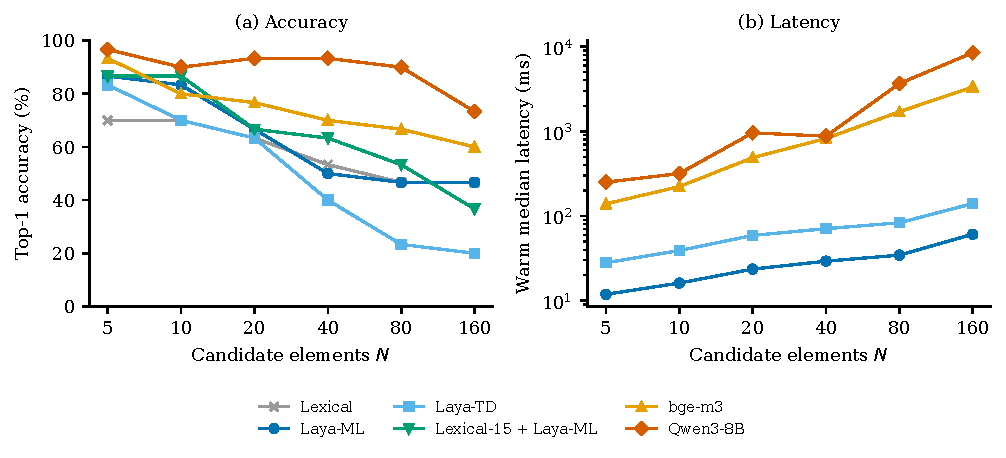
\includegraphics[width=\linewidth]{figures/fig_scaling.pdf}
\caption{Accuracy (a) and warm median latency (b) against the number of candidate links $N$ on a live Wikipedia article (30 trials per point; latency measured with each grounder alone).}\label{fig:scale}
\end{figure}
\begin{table}[t]\centering\small
\begin{tabular}{lrrrrrr}
\toprule
Grounder & $N{=}5$ & $N{=}10$ & $N{=}20$ & $N{=}40$ & $N{=}80$ & $N{=}160$ \\
\midrule
Lexical & 70 & 70 & 63 & 53 & 47 & 47 \\
Laya-ML & 87 & 83 & 67 & 50 & 47 & 47 \\
Laya-TD & 83 & 70 & 63 & 40 & 23 & 20 \\
Lexical-15 + Laya-ML & 87 & 87 & 67 & 63 & 53 & 37 \\
bge-m3 & 93 & 80 & 77 & 70 & 67 & 60 \\
Qwen3-8B & 97 & 90 & 93 & 93 & 90 & 73 \\
\bottomrule
\end{tabular}
\vspace{4pt}\\
\begin{tabular}{lrrrrrr}
\toprule
Grounder & $N{=}5$ & $N{=}10$ & $N{=}20$ & $N{=}40$ & $N{=}80$ & $N{=}160$ \\
\midrule
Laya-ML & 12 & 16 & 24 & 29 & 35 & 61 \\
Laya-TD & 28 & 39 & 59 & 71 & 83 & 140 \\
bge-m3 & 139 & 223 & 489 & 824 & 1704 & 3346 \\
Qwen3-8B & 251 & 318 & 959 & 877 & 3671 & 8490 \\
\bottomrule
\end{tabular}

\caption{Top: accuracy (\%) against $N$. Bottom: warm median latency (ms) from the isolated latency run.}\label{tab:scale}
\end{table}
\begin{table}[t]\centering\small
\begin{tabular}{lrrrrrr}
\toprule
Grounder & $N{=}5$ & $N{=}10$ & $N{=}20$ & $N{=}40$ & $N{=}80$ & $N{=}160$ \\
\midrule
Lexical & 100/40 & 100/40 & 100/27 & 93/13 & 93/0 & 93/0 \\
Laya-ML & 100/73 & 100/67 & 100/33 & 73/27 & 87/7 & 93/0 \\
Laya-TD & 100/67 & 100/40 & 100/27 & 67/13 & 47/0 & 40/0 \\
Lexical-15 + Laya-ML & 100/73 & 100/73 & 100/33 & 80/47 & 80/27 & 73/0 \\
bge-m3 & 100/87 & 100/60 & 100/53 & 100/40 & 100/33 & 100/20 \\
Qwen3-8B & 100/93 & 100/80 & 100/87 & 100/87 & 100/80 & 100/47 \\
\bottomrule
\end{tabular}

\caption{Accuracy (\%) against $N$ as literal/natural (15 trials each per cell).}\label{tab:scalesplit}
\end{table}

\subsection{Confidence and cascades (RQ5)}\label{sec:cascade}
On the 88 discriminative cases Laya-ML's probability was informative: the 42 decisions with $p\ge0.9$ were 88\% correct, the other 46 only 48\% (Table~\ref{tab:conf}, Figure~\ref{fig:rel}). Laya-TD was less confident (31 decisions below 0.5, 45\% correct among them), but all 29 decisions at $p\ge0.9$ were correct. (The 56 easy checkout cases mostly fall into the top bucket and raise the apparent reliability of Laya-ML's high-confidence decisions to 95\%.) We report no calibration metric; the buckets only show that confidence ranks correctness. We evaluated a cascade that escalates to the LLM when $p<\tau$, with $\tau$ chosen leave-one-group-out (Section 3.5) to avoid tuning on test data (Table~\ref{tab:cascade}, Figure~\ref{fig:pareto}). On the 88 cases the Laya-ML cascade reached 78.4\% accuracy with 41\% of decisions escalated at a mean of 141\,ms; the Laya-TD cascade reached 86.4\% with 60\% escalated at 223\,ms; the LLM alone reached 81.8\% at 307\,ms. The Laya-TD cascade was 4.6 points more accurate (4 of 88 cases) and 1.4 times faster than the LLM alone, a difference within noise at this sample size, while the Laya-ML cascade was 3.4 points less accurate and 2.2 times faster. At least one of the four systems (Laya-ML, Laya-TD, embedding, LLM) was correct in 84 of the 88 cases, so routing headroom exists.

\begin{table}[t]\centering\small
\begin{tabular}{lrrrr}
\toprule
Checkpoint (cases) & $p<0.5$ & $0.5$--$0.7$ & $0.7$--$0.9$ & $\geq 0.9$ \\
\midrule
Laya-ML (88 cases) & 11 / 36\% & 10 / 60\% & 25 / 48\% & 42 / 88\% \\
Laya-ML (all 144) & 11 / 36\% & 10 / 60\% & 25 / 48\% & 98 / 95\% \\
Laya-TD (88 cases) & 31 / 45\% & 15 / 80\% & 13 / 77\% & 29 / 100\% \\
Laya-TD (all 144) & 60 / 72\% & 22 / 86\% & 24 / 88\% & 38 / 100\% \\
\bottomrule
\end{tabular}

\caption{Cases (count / accuracy of the top choice) by Laya confidence bucket, on the 88 discriminative cases and on all 144.}\label{tab:conf}
\end{table}
\begin{figure}[t]\centering
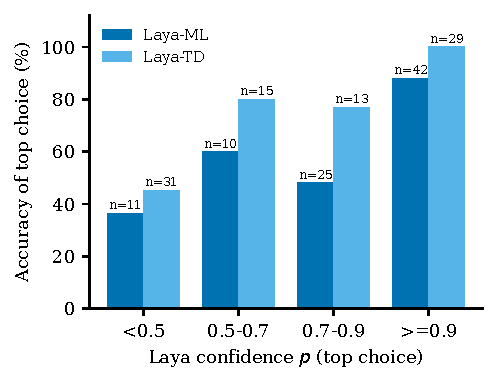
\includegraphics[width=0.52\linewidth]{figures/fig_reliability.pdf}
\caption{Accuracy of the top choice by Laya confidence bucket (88 discriminative cases; counts above bars).}\label{fig:rel}
\end{figure}
\begin{table}[t]\centering\small
\begin{tabular}{lrrrrrr}
\toprule
Configuration & \multicolumn{3}{c}{88 discriminative cases} & \multicolumn{3}{c}{All 144 cases}  \\ \cmidrule(lr){2-4}\cmidrule(lr){5-7} & Escal. & Acc. & ms & Escal. & Acc. & ms \\
\midrule
Laya-ML only & 0\% & 67.0\% & 14 & 0\% & 79.9\% & 14 \\
Laya-ML $\to$ LLM (LOGO) & 41\% & 78.4\% & 141 & 25\% & 86.8\% & 91 \\
Laya-TD only & 0\% & 73.9\% & 44 & 0\% & 84.0\% & 40 \\
Laya-TD $\to$ LLM (LOGO) & 60\% & 86.4\% & 223 & 63\% & 91.7\% & 249 \\
Qwen3-8B only & 100\% & 81.8\% & 307 & 100\% & 88.9\% & 342 \\
\bottomrule
\end{tabular}

\caption{Cascade results. ``LOGO'': threshold chosen on the other suite groups. Escal.\ = share of decisions escalated to the LLM; ms = mean latency per decision. ``Only'' rows use no cascade.}\label{tab:cascade}
\end{table}
\begin{figure}[t]\centering
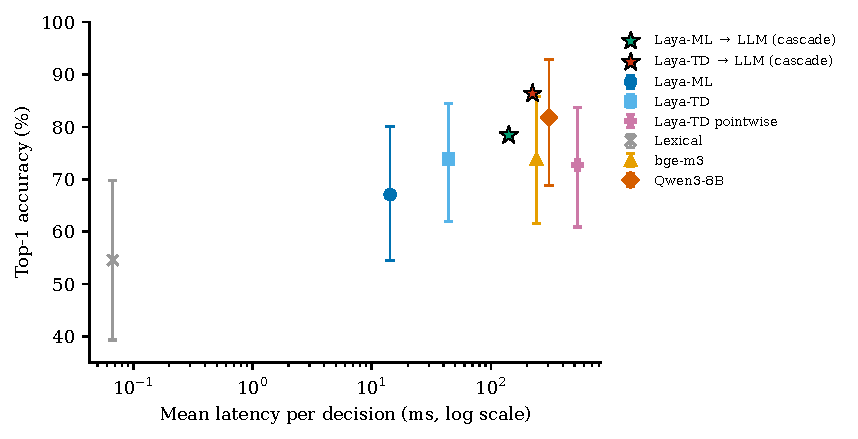
\includegraphics[width=0.78\linewidth]{figures/fig_pareto.pdf}
\caption{Accuracy against mean latency on the 88 discriminative cases for all grounders (error bars: 95\% cluster-bootstrap intervals) and the two cascades (stars, LOGO thresholds).}\label{fig:pareto}
\end{figure}

\subsection{Runtime behaviour (RQ6)}
The idle and batching measurements use a toy three-option routing question (department of a customer message), not a browser decision, with 8 repetitions per idle setting. Latency after an idle gap rose from 8\,ms (back-to-back) to 20\,ms after 0.25\,s and about 50\,ms after two seconds or more (Table~\ref{tab:idle}); a 10\,Hz background ping held it at 19\,ms. A browser agent idles between decisions while pages load, so a realistic per-decision latency is 20--55\,ms; this is consistent with in-situ decisions (median 29--51\,ms across our suites) being slower than isolated ones (14\,ms), although we did not isolate the cause there (Chrome contention is a possible alternative). We did not test the keep-alive inside the full agent loop or measure its power cost. For single UI decisions, the \texttt{compile}, padding and prompt-cache options made no practical difference (16--18\,ms median in all four configurations on 70 real UI decisions; Appendix Table~\ref{tab:compile}). The configurations ran in one process in the listed order, so the one-off 1.2\,s warm-up (the very first call of the first configuration) cannot be attributed to a configuration. Batching helped for bulk decisions: 57 decisions/s at batch size 1 versus about 230 at 16 (Appendix Table~\ref{tab:batch}).

\begin{table}[t]\centering\small
\begin{tabular}{lrr}
\toprule
Idle before call (s) & p50 (ms) & max (ms) \\
\midrule
0 & 8 & 10 \\
0.25 & 20 & 24 \\
0.5 & 24 & 28 \\
1 & 22 & 29 \\
2 & 53 & 62 \\
5 & 49 & 54 \\
10 & 56 & 97 \\
2, with 10\,Hz keep-alive & 19 & 25 \\
\bottomrule
\end{tabular}

\caption{Latency of one Laya-ML decision (toy three-option question) after an idle gap (8 repetitions per row).}\label{tab:idle}
\end{table}

\section{Discussion}
\paragraph{Where Laya fits.} Laya-ML was effective as a structure-tolerant chooser among a shortlist of 3--25 candidates whose labels or row context carry the answer (all live tasks; the checkout flow), and as a fast, offline first stage with informative confidence; identical inputs gave identical decisions on repeated runs on the same machine. It is a poor fit for large undifferentiated candidate lists ($N\ge40$), where it behaved like string matching, for paraphrase-heavy instructions against terse or icon-only UIs, for extracting text it was not given (it chooses among options; values came from quoted strings in our instructions), for planning, and for anything outside the DOM text (closed shadow roots, canvas, pixels).

\paragraph{A layered design (hypothesis, not tested end to end).} The results suggest: (1) a deterministic snapshot across frames and open shadow roots (3--5\,ms); (2) a task-aware shortlist of at most 20--30 candidates (we only tried a crude lexical one, which did not help); (3) a Laya \texttt{choice} question with short labels and descriptions---in a small development probe (Appendix~\ref{app:dev}) bare link text scored 0/4 and label-plus-description 4/4 for Laya-ML, but not for Laya-TD; (4) a confidence gate with LLM or human fallback; (5) a keep-alive while idle; and (6) outcome checks after each step, since a confident choice is not proof of success. For testing, instruction-driven steps complement scripts rather than replace them (Section~4.2).

\paragraph{Sensitivity to formatting and order.} In the development probe the same model scored 0/4 or 4/4 depending only on how options were presented, and a shortlist that only reordered ten candidates changed accuracy by four points; we did not run the same probes on the LLM, so we cannot say whether Laya is more sensitive than an LLM. A held-out validation set is advisable for each new site family.

\paragraph{Cost.} Laya runs locally at no marginal cost per decision. The laya-ultrafast authors report planning calls to a hosted model of about 1--1.5\,s \cite{layaultrafast}, and our local LLM took roughly 0.25--8.5\,s per grounding decision depending on list size; these are different tasks and setups and are not a like-for-like comparison. We did not measure any hosted API.

\section{Limitations}\label{sec:limits}
\begin{itemize}\setlength{\itemsep}{1pt}
\item \textbf{Sample size and dependence.} Slices contain 14--56 cases and scaling cells 30 trials; the cases are not independent (shared fixtures and candidate lists), so intervals are optimistic, and most between-grounder accuracy differences are not significant after correction.
\item \textbf{Post-hoc subset.} The 88 ``discriminative'' cases were defined after observing that all grounders solved the checkout cases; both sets are reported. The cascade threshold was chosen leave-one-group-out with only three or four groups.
\item \textbf{Author-written fixtures, instructions, gold labels and scripted baselines} may favor or disadvantage any method; the scripts were written against variant~A, so their results on C--E are partly by construction; the checkout suite does not discriminate between grounders.
\item \textbf{Laya-ML only end to end.} The executed suites used the 322M model; Laya-TD and the baselines were only replayed on logged cases, so end-to-end claims (including the 94/94 live decisions, which are 18 distinct decisions repeated five times) concern Laya-ML.
\item \textbf{Partial development/held-out separation.} Variant~A was used to choose the option format; later suites were not used for prompt choices, but two harness defects were fixed after seeing live results.
\item \textbf{Modest baselines.} One untuned LLM prompt, one 8B model, one embedding model, a simple lexical scorer; no vision or accessibility-tree agents; browser-specific Laya fine-tunes published by third parties were not tested.
\item \textbf{One machine, one browser, indicative timings.} Apple M2 Pro/16\,GB, headless Chrome 156; swap was partly occupied during some second-protocol runs, LLM latencies varied several-fold between runs, and warm latencies come from a second pass over identical inputs with caches enabled (Section~\ref{sec:env}).
\item \textbf{Independent steps.} Oracle resync and state reset remove error compounding that a real end-to-end agent would suffer.
\item \textbf{Live-site drift and flakiness.} Public sites change; 4 of 95 live steps failed (cause undetermined for three), and the live suite is not held out with respect to the snapshot and checks.
\item \textbf{Related work.} We did not survey the broader literature on web agents and self-healing test automation; comparisons are limited to systems we could run or verify.
\item \textbf{Scaling task.} The Wikipedia natural instructions require world knowledge, which favors the LLM and is not a UI-grounding skill; results at large $N$ come from one article and five targets.
\item \textbf{Unofficial port.} \texttt{laya-mlx} is independent of the model's authors.
\end{itemize}

\section{Conclusion}
Laya-MLX can drive a real browser at interactive speed on a Mac: with a frame-aware snapshot it handled same-origin, cross-origin and nested iframes, open shadow DOM, a duplicate-link table and a third-party app, choosing the right element in all 94 live decisions of Laya-ML (18 distinct decisions repeated five times) at a median of 51\,ms with no network or per-call cost. It is not a general web agent: element-picking accuracy falls steeply with many options (where it behaved like string matching) or paraphrased instructions, and closed shadow roots, canvas and pixels are out of reach. Its confidence, which was informative on our cases, suggests using it as the fast first stage of a layered agent. Next steps are a better candidate shortlist for the $N\ge40$ regime, a keep-alive-aware agent loop, a vision fallback, tests of browser-specific Laya fine-tunes, and in-browser (WebGPU/ONNX) deployment.

\section*{Declarations}
\paragraph{Author contributions.} R.~Keller (sole author): conceptualization, direction of the experiments, validation and responsibility for the final text. Software implementation, analysis and drafting were carried out with AI assistance (see below).
\paragraph{Competing interests.} The author declares no competing interests.
\paragraph{Funding.} No external funding.
\paragraph{Use of AI assistance.} The experimental code, the analysis scripts and the first draft of this manuscript were produced with substantial assistance from an AI coding assistant (Claude, Anthropic) operated by the author. The author is responsible for the content. The AI system is not an author. Every reference was checked against a primary or index source before inclusion.
\paragraph{Ethics.} No human participants or personal data were involved. Automated interaction with third-party sites was limited to public pages intended for, or tolerant of, automation practice (the-internet.herokuapp.com, TodoMVC) and a small number of page loads of one Wikipedia article; no accounts, logins or form submissions with real data were used.
\paragraph{Data and code availability.} The replication package (code, local fixtures, per-decision raw results as JSON, generated tables and figures, and a README) is available at \url{https://github.com/Who-Code/laya-browser-grounding} (directory \texttt{submission/replication}) and archived on Zenodo, DOI \href{https://doi.org/10.5281/zenodo.24004198}{10.5281/zenodo.24004198} (all versions; version 1.0.0: 10.5281/zenodo.24004199). It contains a snapshot of link labels from one Wikipedia article (CC BY-SA 4.0, attribution in the package). Model weights are not redistributed; they are obtained from their original sources under their own licenses.

\begin{thebibliography}{99}\small
\bibitem{laya} Convai Innovations and contributors. \emph{Laya} (decision encoder and weights). GitHub repository \texttt{NandhaKishorM/laya}. \url{https://github.com/NandhaKishorM/laya} (accessed 6 November 2026).
\bibitem{lmlx} GitHub user \texttt{mizorewww}. \texttt{laya-mlx}: open-weight typed decisions on Apple Silicon (independent MLX port), version 0.6.0, Apache-2.0. \url{https://github.com/mizorewww/laya-mlx}; checkpoints \url{https://huggingface.co/aac6fef/laya-mlx} (accessed 6 November 2026).
\bibitem{modernbert} B.~Warner et al. Smarter, better, faster, longer: a modern bidirectional encoder for fast, memory efficient, and long context finetuning and inference. arXiv:2412.13663, 2024 (published at ACL 2025).
\bibitem{mlx} GitHub organization \texttt{ml-explore}. MLX (version 0.32.4 used): an array framework for Apple silicon. \url{https://github.com/ml-explore/mlx} (accessed 6 November 2026).
\bibitem{jev} Browser Use. \emph{jev-ultrafast}. \url{https://github.com/browser-use/jev-ultrafast} (accessed 6 November 2026).
\bibitem{layaultrafast} GitHub user \texttt{ipenywis}. \emph{laya-ultrafast}: a local, open-weight port of jev-ultrafast using Laya. \url{https://github.com/ipenywis/laya-ultrafast} (accessed 6 November 2026).
\bibitem{bgem3} J.~Chen et al. M3-Embedding: multi-linguality, multi-functionality, multi-granularity text embeddings through self-knowledge distillation (the BGE-M3 model). arXiv:2402.03216, 2024.
\bibitem{qwen3} A.~Yang et al. (Qwen Team). Qwen3 technical report. arXiv:2505.09388, 2025.
\bibitem{ollama} Ollama: run large language models locally. \url{https://ollama.com} (accessed 6 November 2026).
\bibitem{playwright} Microsoft. Playwright: reliable end-to-end testing for modern web apps. \url{https://playwright.dev} (accessed 6 November 2026).
\bibitem{theinternet} The Internet (practice site for test automation). \url{https://the-internet.herokuapp.com} (accessed 6 November 2026).
\bibitem{todomvc} TodoMVC: helping you select an MV* framework (React example). \url{https://todomvc.com/examples/react/dist/} (accessed 6 November 2026).
\bibitem{wilson} E.~B. Wilson. Probable inference, the law of succession, and statistical inference. \emph{Journal of the American Statistical Association}, 22(158):209--212, 1927.
\end{thebibliography}

\appendix
\section{Prompts and question formats}\label{app:prompts}
\paragraph{Laya choice.} State = the instruction. Question (instructions field): \emph{``Which interface element should be used to carry out this instruction?''} Options: \texttt{\{label: description\}} with label = element name (at most 60 characters; row context or an ordinal ``(k of n)'' appended on collision) and description = \texttt{role 'name' in 'row context'}.
\paragraph{Laya pointwise.} For each candidate: state = \texttt{Instruction: <instruction>} newline \texttt{Element: <description>}; yes/no (\texttt{noul}) question \emph{``Is this the element the instruction refers to?''}; the candidate with the highest $P(\text{true})$ is chosen.
\paragraph{Select options.} Options = the visible option texts; question \emph{``Which option should be selected?''}
\paragraph{LLM.} One user message, via the Ollama chat interface with thinking disabled, temperature 0, at most 8 output tokens:
\begin{quote}\small\ttfamily
Page elements:\\ {[0]} <description>\\ {[1]} <description>\\ \ldots\\[2pt] Instruction: <instruction>\\ Which element number should be acted on? Answer with only the number.
\end{quote}
\paragraph{Embedding.} One batched request embedding the instruction and all candidate descriptions with \texttt{bge-m3}; the candidate with the highest cosine similarity is chosen.
\paragraph{Lexical.} Tokens are lowercased alphanumeric words, stop words removed, truncated to six characters. A candidate's score sums $\log(1+n/\mathrm{df}_w)$ over instruction tokens present in its text (extra weight $0.4\times$ for tokens in its name), $n$ = number of candidates.

\section{Instruction sets}\label{app:instr}
\begin{table}[ht]\centering\small\begin{tabular}{@{}lp{5.4cm}p{5.6cm}@{}}
\toprule
Step & Literal instruction & Natural instruction \\
\midrule
type & Type \textquotesingle{}Call mom\textquotesingle{} into the What needs to be done? field & Type \textquotesingle{}Call mom\textquotesingle{} into the new task box \\
add & Click Add & Submit the new task \\
toggle & Check the Walk dog checkbox & Tick off \textquotesingle{}Walk dog\textquotesingle{} \\
delete & Click Delete on Write report & Get rid of the \textquotesingle{}Write report\textquotesingle{} item \\
f\_active & Click the Active filter & Show only the tasks that are still open \\
f\_all & Click the All filter & Show every task again \\
clear & Click Clear completed & Remove all the finished tasks \\
\bottomrule
\end{tabular}
\caption{Todo suite instructions.}\end{table}
\begin{table}[ht]\centering\small\begin{tabular}{@{}lp{11cm}@{}}
\toprule
Step & Instruction \\
\midrule
add\_blue & Add the blue mug to the cart \\
checkout & Go to checkout \\
holder & Enter \textquotesingle{}Ada Lovelace\textquotesingle{} as the cardholder name \\
cardno & Type \textquotesingle{}1234 5678 9012 3456\textquotesingle{} into the card number field \\
country & Choose Germany as the country \\
pay & Pay now \\
\bottomrule
\end{tabular}
\caption{Checkout suite instructions (dummy field values).}\end{table}
\begin{table}[ht]\centering\small\begin{tabular}{@{}llp{9.4cm}@{}}
\toprule
Task & \# & Instruction \\
\midrule
checkboxes & 1 & Tick the first checkbox \\
checkboxes & 2 & Untick the second checkbox \\
dropdown & 1 & Choose Option 2 from the dropdown list \\
add\_remove & 1 & Click Add Element \\
add\_remove & 2 & Remove the element you just added \\
dynamic\_loading & 1 & Start the loading process \\
js\_alerts & 1 & Trigger the JS confirm dialog \\
inputs & 1 & Type \textquotesingle{}42\textquotesingle{} into the number input \\
status\_codes & 1 & Open the page for status code 404 \\
challenging\_dom & 1 & Click the edit link in the table row for \textquotesingle{}Iuvaret5\textquotesingle{} \\
challenging\_dom & 2 & Click the delete link in the table row for \textquotesingle{}Apeirian7\textquotesingle{} \\
tinymce\_iframe & 1 & Type \textquotesingle{}Hello from Laya\textquotesingle{} into the text editor \\
todomvc\_react & 1 & Type \textquotesingle{}Buy milk\textquotesingle{} into the new todo input and press Enter \\
todomvc\_react & 2 & Type \textquotesingle{}Walk dog\textquotesingle{} into the new todo input and press Enter \\
todomvc\_react & 3 & Type \textquotesingle{}Write report\textquotesingle{} into the new todo input and press Enter \\
todomvc\_react & 4 & Mark \textquotesingle{}Walk dog\textquotesingle{} as done \\
todomvc\_react & 5 & Show only the active items \\
todomvc\_react & 6 & Show only the finished items \\
todomvc\_react & 7 & Clear the finished items \\
\bottomrule
\end{tabular}
\caption{Live suite instructions.}\end{table}

\section{Development probes}\label{app:dev}
These probes were run during development, on an earlier snapshot version, before the final protocol; they are reported for transparency and were not re-run. \emph{Link probe:} on a local help-center page with 15 links and four goals, options given as (A) bare link text, (B) ``link $i$'' labels with the link text as description, (C) short title with the link text as description: Laya-ML scored 0/4, 3/4 and 4/4; Laya-TD scored 3/4, 2/4 and 3/4. \emph{Todo variant~A (14 cases):} option formats (A) name, (B) ``Button labeled \ldots'', (C) name plus role and row in parentheses, under two question wordings, gave 9--10/14 for Laya-ML in all six combinations; the pointwise yes/no formulation gave 8--9/14 (Laya-ML) and 10--12/14 (Laya-TD). These probes did not discriminate well between formats for Laya-ML on the development set (9--10/14 in all combinations), and the link probe has only four questions and favors label-plus-description for Laya-ML but not for Laya-TD; we nevertheless kept the label-plus-description choice format and the first question wording for all later suites.

\section{Paired comparisons}
\begin{table}[h]\centering\small\begin{tabular}{lrrrr}
\toprule
A $-$ B & Diff.\ (points) & 95\% CI & $p$ & $p_{\mathrm{Holm}}$ \\
\midrule
Laya-TD $-$ Lexical & +19.3 & [+8.3, +31.0] & 0.0046 & 0.070 \\
Qwen3-8B $-$ Lexical & +27.3 & [+10.7, +44.2] & 0.0083 & 0.116 \\
bge-m3 $-$ Lexical & +19.3 & [+6.2, +32.1] & 0.0112 & 0.146 \\
Laya-ML $-$ Lexical & +12.5 & [+3.3, +23.6] & 0.0269 & 0.323 \\
Laya-TD pointwise $-$ Lexical & +18.2 & [+3.4, +33.0] & 0.0413 & 0.454 \\
Qwen3-8B $-$ Laya-ML & +14.8 & [-1.2, +30.2] & 0.1359 & 1.000 \\
bge-m3 $-$ Laya-ML & +6.8 & [-2.8, +15.5] & 0.2711 & 1.000 \\
Qwen3-8B $-$ Laya-TD pointwise & +9.1 & [-7.6, +25.0] & 0.3635 & 1.000 \\
Qwen3-8B $-$ Laya-TD & +8.0 & [-7.0, +22.7] & 0.4027 & 1.000 \\
Laya-TD $-$ Laya-ML & +6.8 & [-6.9, +18.8] & 0.4259 & 1.000 \\
Laya-TD pointwise $-$ Laya-ML & +5.7 & [-5.6, +15.7] & 0.4305 & 1.000 \\
Qwen3-8B $-$ bge-m3 & +8.0 & [-9.5, +25.0] & 0.4700 & 1.000 \\
Laya-TD pointwise $-$ Laya-TD & -1.1 & [-14.5, +13.0] & 1.0000 & 1.000 \\
bge-m3 $-$ Laya-TD & +0.0 & [-12.0, +13.8] & 1.0000 & 1.000 \\
bge-m3 $-$ Laya-TD pointwise & +1.1 & [-7.5, +10.2] & 1.0000 & 1.000 \\
\bottomrule
\end{tabular}

\caption{All 15 grounder pairs on the 88 discriminative cases: difference in accuracy, 95\% instruction-level (cluster) bootstrap interval, sign-flip permutation $p$ over 32 instructions, and Holm-adjusted $p$.}\label{tab:paired}\end{table}

\section{Additional runtime results}
\begin{table}[ht]\centering\small\begin{tabular}{lrrrrr}
\toprule
Configuration & 1st p50 & 1st p95 & 1st max & 2nd p50 & 2nd p95 \\
\midrule
default & 18 & 24 & 1164 & 18 & 20 \\
compile & 17 & 23 & 30 & 16 & 18 \\
compile+pad16 & 16 & 20 & 29 & 17 & 20 \\
compile+pad16+cache & 16 & 21 & 31 & 17 & 20 \\
\bottomrule
\end{tabular}

\caption{Laya-ML configuration comparison (``default'' = no compile, padding or cache flags): median and 95th percentile (ms) of 70 real UI decisions, first and second pass; ``max'' is the slowest first-pass call. Configurations ran in this order in one process.}\label{tab:compile}\end{table}
\begin{table}[ht]\centering\small\begin{tabular}{lrr}
\toprule
Batch size & p50 per batch (ms) & Decisions/s \\
\midrule
1 & 18 & 57 \\
4 & 21 & 193 \\
16 & 69 & 231 \\
64 & 319 & 201 \\
\bottomrule
\end{tabular}

\caption{Batched three-way routing of customer messages (toy task) with Laya-ML.}\label{tab:batch}\end{table}

\end{document}
